\svnid{$Id$}
\section{Command Line Interface}
\subsection{Command overview} \label{fr:Batch interface-Command overview}
For almost every command, either a long or a short version can be used. These commands can be used by \code{codecover \%\textbf{command}\% [\%options\%]}.
\begin{longtable}{|l|p{6cm}|}\hline
   {\textbf{Command}} &
   {\textbf{Description}} \\\hline \hline \endhead
   \ref{Command-Instrumenter-Info}: {ii, instrumenter-info} & get information of all available instrumenters \\\hline
   \ref{Command-Instrument}: {in, instrument} & instrumentation of code files \\\hline
   \ref{Command-Analyze}: {an, analyze} & Analysis of a coverage run to create a test-session \\\hline
   \ref{Command-Report}: {re, report} & Generating a report from a test-session \\\hline
   \ref{Command-Info}: {info} & Showing the information of a test-session container and the contained test-sessions and test cases \\\hline
   \ref{Command-Merge-Sessions}: {ms, merge-sessions} & Merging two or more test-sessions \\\hline
   \ref{Command-Alter-Session}: {as, alter-session} & Altering test-session information \\\hline
   \ref{Command-Copy-Sessions}: {cs, copy-sessions} & Copy test-sessions from one session container to another \\\hline
   \ref{Command-Remove-Sessions}: {rs, remove-sessions} & Removing test-sessions from a session container \\\hline
   \ref{Command-Merge-Test-Cases}: {mt, merge-test-cases} & Merging two or more test cases \\\hline
   \ref{Command-Alter-Test-Case}: {at, alter-test-case} & Editing test case information \\\hline
   \ref{Command-Remove-Test-Cases}: {rt, remove-test-cases} & Removing test cases from a session container \\\hline
   \ref{Command-Help}: {h, help} & A help page containing this command overview or an option and parameter overview a given command. \\\hline

  \caption{Command line interface command overview}
  \label{CLI command overview}
\end{longtable}

%%%%%%%%%%%%%%%%%%%%%%%%%%%%%%%%%%%%%
%%%%%%%%%%%%  General Commands  %%%%%
%%%%%%%%%%%%%%%%%%%%%%%%%%%%%%%%%%%%%
\subsection{General Commands}\label{General}
For every command a set of options is supported. In addition to specific command options, all commands support some global parameterless options. They are not required but change the behavior of the software when used. These commands can be used by \code{codecover \%command\% [\%\textbf{options}\%]}.
\begin{longtable}{|l|p{8cm}|}\hline
   {\textbf{Option}} &
   {\textbf{Explanation}} \\\hline \hline \endhead
     \verb$-v, --verbose$ & Orders the software to print more information as usual. For example this can be a description of the actions being done. This option is the opposite of \verb$--quiet$. \\\hline
     \verb$-q, --quiet$ & Orders the software not to print information to the shell. This option is the opposite to \verb$--verbose$. \\\hline
     \verb$-p, --pretend$ & Orders the software not to perform any actions affecting the data persistently but to print information about what the software would do instead. Using \verb$--pretend$ the actor can make sure that his command has the correct syntax and would be successfully executed. \\\hline
     \verb$-h, --help$ & Prints an option and parameter overview of the given command. Has the same effect like \verb$codecover help \%command\%$. \\\hline
     \verb$-V, --version$ & Prints out the version of the software. Has the same effect like \verb$codecover --version$. \\\hline
  \caption{General batch options}
  \label{fr_tb:General batch command options}
\end{longtable}

%%%%%%%%%%%%%%%%%%%%%%%%%%%%%%%%%%%%%
%%%%%%%%  Instrumenter-Info %%%%%%%%%
%%%%%%%%%%%%%%%%%%%%%%%%%%%%%%%%%%%%%
\subsection{Instrumenter-Info}\label{Command-Instrumenter-Info}
This command is used to get information of all available instrumenters. If there are two or more instrumenters available for a given programming language, you can get to know the unique keys of the possible instrumenters. These key can than be used for the option \code{instrumenter} of the instrument command (\ref{Command-Instrument}).

\subsubsection{Usage}\label{command:ii:usage}
\begin{quote}
\code{codecover (instrumenter-info|ii) [options]}
\end{quote}

\subsubsection{Options}\label{command:ii:options}
\seealso{\nameref{General}}
The following table lists all the options, that are available for use with this command.
%\begin{maxipage}
\begin{longtable}{|l|p{4cm}|}\hline
   {\textbf{Option}} & 
   {\textbf{Description}} \\\hline \hline \endhead
   \verb$-l, --language <lang>$ & (\code{java}|\code{cobol}) \\\hline
  \caption{Options for command instrumenter-info}
  \label{fr_tb:Options for command instrumenter-info}
\end{longtable}

\subsubsection{Examples}\label{command:ii:examples}
\begin{quote}
\begin{verbatim}
codecover instrumenter-info -l java
                            -v
\end{verbatim}
\end{quote}
Print out verbose information of all instrumenters, that support the programming language java.

%%%%%%%%%%%%%%%%%%%%%%%%%%%%%%%%%%%%%
%%%%%%%%%%%%  Instrument %%%%%%%%%%%%
%%%%%%%%%%%%%%%%%%%%%%%%%%%%%%%%%%%%%
\subsection{Instrument}\label{Command-Instrument}
This command is used to instrument source code files so that the coverage will be measured when these files will be executed.
\subsubsection{Usage}\label{command:in:usage}
\begin{quote}
\code{codecover (instrument|in) [options]}
\end{quote}

\subsubsection{Options}\label{command:in:options}
\seealso{\nameref{General}}
The following table lists all the options, that are available for use with this command.
%\begin{maxipage}
\begin{longtable}{|l|p{4cm}|c|}\hline
   {\textbf{Option}} & 
   {\textbf{Description}} & 
   {\textbf{Required}} \\\hline \hline \endhead
   \verb$-r, --root-directory <dir>$ & the root directory of the source files & \x \\\hline
   \verb$-i, --include <pattern>$ & a relative include pattern; this argument can occur more than one time &  \\\hline
   \verb$-f, --includes-file <file>$ & a file containing a list of relative include patterns separated by new line & \\\hline
   \verb$-e, --exclude <pattern>$ & a relative exclude pattern; this argument can occur more than one time & \\\hline
   \verb$-x, --excludes-file <file>$ & a file containing a list of relative exclude patterns separated by new line & \\\hline
   \verb$-o, --criterion <crit>$ & one of (\code{all}, \code{st}, \code{br}, \code{co}, \code{lo}); this argument can occur more than one time -- once for every criterion & \\\hline
   \verb$-l, --language <lang>$ & (\code{java}|\code{cobol}) & \x \\\hline
   \verb$-I, --instrumenter <key>$ & the unique key of the instrumenter to use; use the command \code{instrumenter-info} (\ref{Command-Instrumenter-Info}) to get the correct key & \\\hline
   \verb$-d, --destination <dir>$ & the destination directory for the instrumented files & \x \\\hline
   \verb$-c, --container <file>$ & the new session container & \x \\\hline
   \verb$-a, --charset <charset>$ & the character encoding of the source files & \\\hline
   \verb$-u, --copy-uninstrumented$ & advices the software to copy all files of the root-directory, that where not instrumented, to the destination & \\\hline
   \verb$-D, --directive$ & arguments of the style \code{key=value} to enable special features of the instrumenter; the instrumenter-info command prints out a list of directives, an instrumenter supports  & \\\hline
  \caption{Options for command instrument}
  \label{fr_tb:Options for command instrument}
\end{longtable}
%\end{maxipage}

The arguments of option \code{criteria} stand for:
\begin{longtable}{|c|l|}\hline
   {\textbf{Criteria abbreviation}} &
   {\textbf{Explanation}} \\\hline \hline \endhead
     \code{all} & all criteria \\\hline
     \code{st} & statement coverage \\\hline
     \code{br} & branch coverage \\\hline
     \code{co} & condition coverage \\\hline
     \code{lo} & loop coverage \\\hline
  \caption{Explanation of the criteria abbreviations}
  \label{fr_tb:Explanation of the criteria abbreviations}
\end{longtable}

\subsubsection{Patterns}
For a more detailed selection, include and exclude patterns can be used. These patterns allow wildcards and are adopted from the \linkwithfootnote{http://ant.apache.org/}{apache ant project} (see their  \linkwithfootnote{http://ant.apache.org/manual/dirtasks.html}{pattern description}).
\par
The wildcard \code{?} matches one character. The wildcard \code{*} matches zero or more characters. Examples:
\begin{itemize}
\item \code{?.java} matches  \code{x.java} and \code{A.java}, but not \code{.java} or \code{xyz.java} (both don't have one character before \code{.java}).
\item \code{*.java}  matches \code{.java}, \code{x.java} and \code{FooBar.java}, but not \code{FooBar.xml} (does not end with \code{.java}).
\end{itemize}
Combinations of \code{*}'s and \code{?}'s are allowed.
\par
To match a complete directory tree, or a file anywhere in the directory tree, use \code{**}. When \code{**} is used as the name of a directory in the pattern, it matches zero or more directories. Example:
\begin{itemize}
\item \code{src/**/*.java} matches all java files under \code{src/}, such as \code{src/x.java}, or \code{src/foo/bar/MyObject.java}, but not \code{Main.java} or \code {test/AllTests.java} (Do not lie under \code{test}).
\end{itemize}
\par
The instrumenter uses some ignore patterns for files, that are totally ignored:
\begin{itemize}
\item \verb$**/*~, **/#*#, **/.#*, **/%*%", **/._*"$
\item \verb$**/.svn/**, **/_svn/**, **/CVS/**, **/.cvsignore$
\item \verb$**/SCCS/**, **/vssver.scc, **/.DS_Store, **/Thumbs.db$
\end{itemize}

\subsubsection{Examples}\label{command:in:examples}
\begin{quote}
\begin{verbatim}
codecover instrument -r src/ 
                     -d bin/instr/ 
                     -c container.xml 
                     -l java
\end{verbatim}
\end{quote}
Find all java source files in the directory "src", parse and instrument these files into the directory "bin/instr/". The source files are instrumented for all criteria and the static information compiled during the instrumentation is stored in the "container.xml".  
\begin{quote}
\begin{verbatim}
codecover instrument -r src/ 
                     -d bin/instr/ 
                     -i "org/pak1/**"
                     -e "**/*Test.java"
                     -c container.xml 
                     -l java
                     -I CodeCover_Java_1.5
                     -o st lo
                     -a UTF-8
                     -u
\end{verbatim}
\end{quote}
Find all java source files under the directory "org/pak1", exclude files ending with "Test.java", parse these files with the "UTF-8" charset and instrument them into the directory "bin/instr/". The source files are instrumented for statement and loop coverage, and the static information compiled during the instrumentation is stored in the "container.xml". All files under "src", which are not instrumented, are copied to "bin/instr/". The code cover instrumenter for java is used. It is specified by its unique key \textit{CodeCover\_Java\_1.5}.


%%%%%%%%%%%%%%%%%%%%%%%%%%%%%%%%%%%%%
%%%%%%%%%%%%%% Analyze %%%%%%%%%%%%%%
%%%%%%%%%%%%%%%%%%%%%%%%%%%%%%%%%%%%%
\subsection{Analyze}\label{Command-Analyze}
This command is used to import a coverage-log, that was produced by an instrumented program, into a specified test-session container.
\subsubsection{Usage}\label{command:an:usage}
\begin{quote}
\code{codecover (analyze|an) [options]}
\end{quote}

\subsubsection{Options}\label{command:an:options}
\seealso{\nameref{General}}
The following table lists all the options, that are available for use with this command.
\begin{longtable}{|l|p{4cm}|c|}\hline
   {\textbf{Option}} & 
   {\textbf{Description}} & 
   {\textbf{Required}} \\\hline \hline \endhead
   \verb$-c, --container <file>$ & the test-session container the coverage data should be added to & \x \\\hline
   \verb$-g, --coverage-log <file>$ & the coverage log produced by the executed program & \x  \\\hline
   \verb$-n, --name <name>$ & the name of the new test-session containing the coverage results & \x \\\hline
   \verb$-m, --comment <text>$ & a comment describing the test-session & \\\hline
   \verb$-a, --charset <charset>$ & the character encoding of the coverage log file & \\\hline
  \caption{Options for command analyze}
  \label{fr_tb:Options for command analyze}
\end{longtable}

\subsubsection{Examples}\label{command:an:examples}
\begin{quote}
\begin{verbatim}
codecover analyze -c container.xml
                  -g coverageLog.clf
                  -n "test-session 1" 
\end{verbatim}
\end{quote}
Load the test-session container from "container.xml", as well as parse the generated coverage log "coverageLog.clf", and add the data contained in the coverage log to the test-session container under the name "test-session 1".
\begin{quote}
\begin{verbatim}
codecover analyze -c container.xml 
                  -g coverageLog2.clf 
                  -n "test-session 2"
                  -m "Another test-session"
\end{verbatim}
\end{quote}
Load the test-session container from "container.xml", as well as parse the generated coverage log "coverageLog2.clf", and add the data contained in the coverage log to the test-session container under the name "test-session 2" and the comment "Another test-session".

%%%%%%%%%%%%%%%%%%%%%%%%%%%%%%%%%%%%%
%%%%%%%%%%%%%% Report  %%%%%%%%%%%%%%
%%%%%%%%%%%%%%%%%%%%%%%%%%%%%%%%%%%%%
\subsection{Report}\label{Command-Report}
Creates a report of a test-session. A template which specifies the appearance and format is used to generate the report.
\subsubsection{Usage}\label{command:re:usage}
\begin{quote}
\code{codecover (report|re) [options]}
\end{quote}

\subsubsection{Options}\label{command:re:options}
\seealso{\nameref{General}}
The following table lists all the options, that are available for use with this command.
\begin{longtable}{|l|p{4cm}|c|}\hline
   {\textbf{Option}} & 
   {\textbf{Description}} & 
   {\textbf{Required}} \\\hline \hline \endhead
   \verb$-c, --container <file>$ & the session container to use & \x \\\hline
   \verb$-s, --session <name>$ & the name of the test-session for the report & \x \\\hline
   \verb$-p, --template <file>$ & the template file containing transformation descriptions & \x \\\hline
   \verb$-d, --destination <file>$ & the destination for the report & \x \\\hline
  \caption{Options for command report}
  \label{fr_tb:Options for command report}
\end{longtable}

\subsubsection{Examples}\label{command:re:examples}
%\begin{fullpage}

\begin{figure}[htbp]
\begin{center}
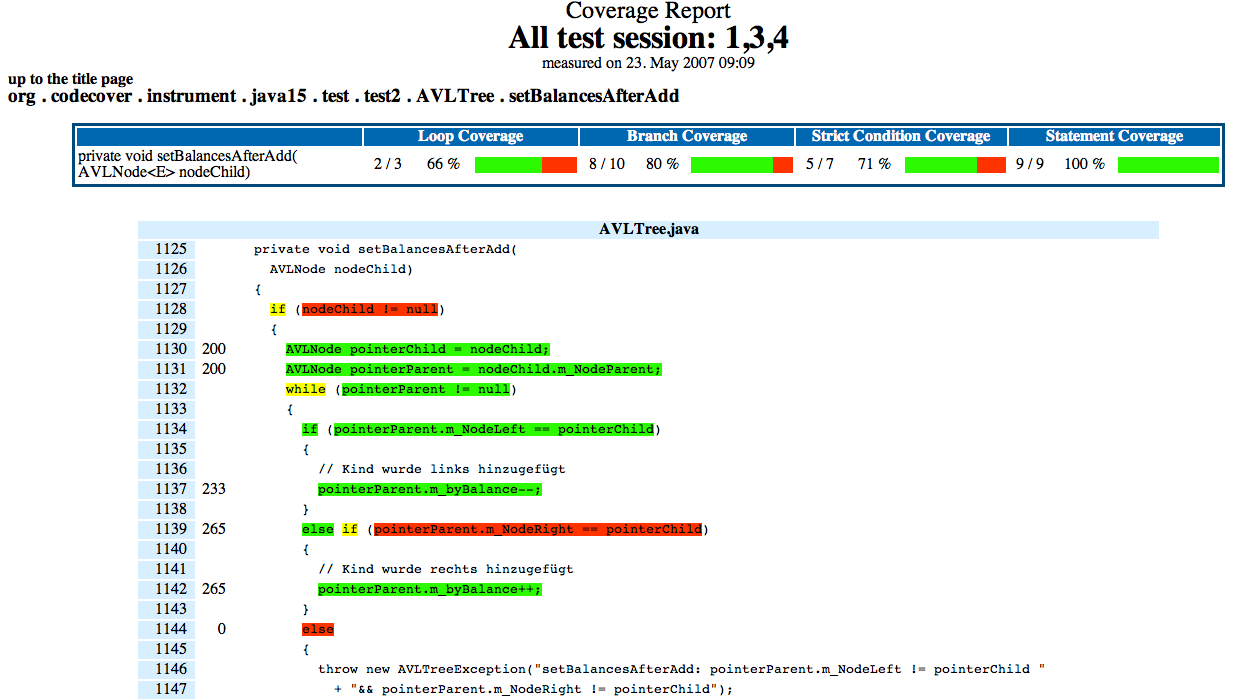
\includegraphics[width = \textwidth]{images/report_example.png}
\caption{An example CodeCover report}
\label{command:re:fig:example}
\end{center}
\end{figure}

%\end{fullpage}


%%%%%%%%%%%%%%%%%%%%%%%%%%%%%%%%%%%%%
%%%%%%%%%%%%%   Info   %%%%%%%%%%%%%%
%%%%%%%%%%%%%%%%%%%%%%%%%%%%%%%%%%%%%
\subsection{Info}\label{Command-Info}
Shows information about a test-session container. The options allow to manipulate the output, as detailed in \ref{command:info:examples}~\nameref{command:info:examples}
\subsubsection{Usage}\label{command:info:usage}
\begin{quote}
\code{codecover info [options]}
\end{quote}

\subsubsection{Options}\label{command:info:options}
\seealso{\nameref{General}}
The following table lists all the options, that are available for use with this command.\\

\begin{longtable}{|l|p{4cm}|c|}\hline
   {\textbf{Option}} & 
   {\textbf{Description}} & 
   {\textbf{Required}} \\\hline \hline \endhead
   \verb$-c, --container <file>$ & the test-session container & \x \\\hline
   \verb$-s, --session <name>$ & the name of a test-session &  \\\hline
   \verb$-t, --test-cases$ & showing test case information &  \\\hline
  \caption{Options for command info}
  \label{fr_tb:Options for command info}
\end{longtable}
\subsubsection{Examples}\label{command:info:examples}
\marginlabel{General example}
The following shows the different information levels \codecover provides. Calling the info command with only the test-session container, results in a list of all the test-session contained in this test-session container, with their name, and the date, they were created on. By naming test-sessions present in the test-session container, you can tailor the output to your specific needs.

\begin{verbatim}
root@deepthought:~> codecover info -c container.xml
---------------------------------------------------------------------
test-session container: container.xml

test-sessions:
name         | date                                        
---------------------------------------------------------------------
TestSession0 | 2007-05-18 17:47:32 +0200 (Fri, 18 May 2007)
TestSession1 | 2007-05-18 17:47:32 +0200 (Fri, 18 May 2007)
TestSession2 | 2007-05-18 17:47:32 +0200 (Fri, 18 May 2007)
---------------------------------------------------------------------	
\end{verbatim}

\marginlabel{Example with \code{verbose}}
Adding "verbose" as an option to the above call, additionally displays the comment of the test-sessions in the test-session container.

\begin{verbatim}
root@deepthought:~> codecover info --verbose
                                   -c container.xml
---------------------------------------------------------------------
test-session container: container.xml

test-sessions:
name         | date                                         | comment
---------------------------------------------------------------------
TestSession0 | 2007-05-18 17:47:32 +0200 (Fri, 18 May 2007) | 42
TestSession1 | 2007-05-18 17:47:32 +0200 (Fri, 18 May 2007) | 42
TestSession2 | 2007-05-18 17:47:32 +0200 (Fri, 18 May 2007) | 42
---------------------------------------------------------------------
\end{verbatim}

\marginlabel{Example with \code{test-cases}}
Calling the info command with the "test-cases" option results in a more detailed break-down of the test-session container. Each test-session is listed, as well as a list of all the test cases contained in it. This list of test cases provides the name of the test case and its creation date.

\begin{verbatim}
root@deepthought:~> codecover info --test-cases 
                                   -c container.xml 
                                   -s TestSession0
---------------------------------------------------------------------
test-session container: container.xml
=====================================================================
test-session name:    TestSession0
test-session date:    2007-05-18 17:47:32 +0200 (Fri, 18 May 2007)
test-session comment: 42

test cases:
name        | date                                        
---------------------------------------------------------------------
TestCase0   | 2007-05-18 17:47:32 +0200 (Fri, 18 May 2007)
TestCase99  | 2007-05-18 17:47:32 +0200 (Fri, 18 May 2007)
TestCase198 | 2007-05-18 17:47:32 +0200 (Fri, 18 May 2007)
TestCase297 | 2007-05-18 17:47:32 +0200 (Fri, 18 May 2007)
---------------------------------------------------------------------
\end{verbatim}

\marginlabel{Example with \code{test-cases} and \code{verbose}}
As before, calling the info command with "test-cases" option, as well as the "verbose" option, adds the comments to the list of test cases in the given test-session

\begin{verbatim}
root@deepthought:~> codecover info --verbose 
                                   --test-cases 
                                   -c container.xml 
                                   -s TestSession0
---------------------------------------------------------------------
test-session container: container.xml
=====================================================================
test-session name:    TestSession0
test-session date:    2007-05-18 17:47:32 +0200 (Fri, 18 May 2007)
test-session comment: 42

test cases:
name        | date                                         | comment
---------------------------------------------------------------------
TestCase0   | 2007-05-18 17:47:32 +0200 (Fri, 18 May 2007) | 42
TestCase99  | 2007-05-18 17:47:32 +0200 (Fri, 18 May 2007) | 42
TestCase198 | 2007-05-18 17:47:32 +0200 (Fri, 18 May 2007) | 42
TestCase297 | 2007-05-18 17:47:32 +0200 (Fri, 18 May 2007) | 42
---------------------------------------------------------------------
\end{verbatim}


%%%%%%%%%%%%%%%%%%%%%%%%%%%%%%%%%%%%%
%%%%%%%%%%  Merge Sessions  %%%%%%%%%
%%%%%%%%%%%%%%%%%%%%%%%%%%%%%%%%%%%%%
\subsection{Merge Sessions}\label{Command-Merge-Sessions}
This command is used to merge one or more test-sessions of a session container into a new test-session.
\subsubsection{Usage}\label{command:ms:usage}
\begin{quote}
\code{codecover (merge-sessions|ms) [options]}
\end{quote}

\subsubsection{Options}\label{command:ms:options}
\seealso{\nameref{General}}
The following table lists all the options, that are available for use with this command.
\begin{longtable}{|l|p{4cm}|c|}\hline
   {\textbf{Option}} & 
   {\textbf{Description}} & 
   {\textbf{Required}} \\\hline \hline \endhead
   \verb$-c, --container <file>$ & the session container to use & \x \\\hline
   \verb$-s, --session <name>$ & a name of a test-session participating in the merging; this argument can occur more than one time -- once for every participant & \x \\\hline
   \verb$-r, --remove-old-test-sessions$ & indicates, whether or not the test-sessions, that were merged, are removed after merging & \\\hline
   \verb$-n, --name <name>$ & the name of the merged test-session & \x \\\hline
   \verb$-m, --comment <text>$ & a comment describing the merged test-session & \\\hline
  \caption{Options for command merge-sessions}
  \label{fr_tb:Options for command merge-sessions}
\end{longtable}

\subsubsection{Examples}\label{command:ms:examples}
\begin{quote}
\begin{verbatim}
codecover merge-sessions -c container.xml 
                         -n "Merged test-session" 
                         -s "test-session 1" "test-session 2" 
\end{verbatim}
\end{quote}
Loads the test-session container from the file "container.xml" and merges the two test-sessions "test-session 1" and "test-session 2" into the new "Merged test-session". By default the merged test-sessions - "test-session 1" and "test-session 2" - are \emph{not} deleted.
\begin{quote}
\begin{verbatim}
codecover merge-sessions --remove-old-test-sessions 
                         -c container.xml 
                         -s "test-session 1" "test-session 2"
                         -n "Merged test-session" 
\end{verbatim}
\end{quote}
Adding the "remove-old-test-sessions" to the command performs the operation described above, but deletes the merged test-sessions - "test-session 1" and "test-session 2" - from the test-session container.
%%%%%%%%%%%%%%%%%%%%%%%%%%%%%%%%%%%%%
%%%%%%%%%%% Alter Session %%%%%%%%%%%
%%%%%%%%%%%%%%%%%%%%%%%%%%%%%%%%%%%%%
\subsection{Alter Session}\label{Command-Alter-Session}
This command is used to modify the name and/or the comment of a test-session.
\subsubsection{Usage}\label{command:as:usage}
\begin{quote}
\code{codecover (alter-session|as) [options]}
\end{quote}

\subsubsection{Options}\label{command:as:options}
\seealso{\nameref{General}}
The following table lists all the options, that are available for use with this command.
\begin{longtable}{|l|p{4cm}|c|}\hline
   {\textbf{Option}} & 
   {\textbf{Description}} & 
   {\textbf{Required}} \\\hline \hline \endhead
   \verb$-c, --container <file>$ & the session container to use & \x \\\hline
   \verb$-s, --session <name>$ & the old name of the test-session & \x \\\hline
   \verb$-n, --name <name>$ & a new name of the test-session & \\\hline
   \verb$-m, --comment <text>$ & a new comment describing the test-session & \\\hline
  \caption{Options for command alter-session}
  \label{fr_tb:Options for command alter-session}
\end{longtable}

\subsubsection{Examples}\label{command:as:examples}
\begin{quote}
\begin{verbatim}
codecover alter-session -c container.xml 
                        -s "Session 1"
                        -n "New Name" 
                        -m "New Comment"
\end{verbatim}
\end{quote}
Load the test-session container from "container.xml", rename the test-session with the name "Session 1" to "New Name" and change the comment of it to "New Comment". The option for the comment is not required, so a test-session can be renamed without changing its comment.

%%%%%%%%%%%%%%%%%%%%%%%%%%%%%%%%%%%%%
%%%%%%%%%%%% Copy Sessions %%%%%%%%%%
%%%%%%%%%%%%%%%%%%%%%%%%%%%%%%%%%%%%%
\subsection{Copy Sessions}\label{Command-Copy-Sessions}
This command is used to copy one or more test-sessions from one session container to another. \newline
\attention
If the destination test-session container does not exists, the source test-session container is copied to the location of the destination test-session container, while containing only the specified test-sessions.\newline
\attention
If the destination test-session container already contains a test-session, that is to be copied into it, from the source test-session container, the copied test-session is renamed along the lines of "Test Session" to "Test Session (1)". The test-session that was already present in the destination test-session container is not modified. 

\subsubsection{Usage}\label{command:cs:usage}
\begin{quote}
\code{codecover (copy-sessions|cs) [options]}
\end{quote}

\subsubsection{Options}\label{command:cs:options}
\seealso{\nameref{General}}
The following table lists all the options, that are available for use with this command.
\begin{longtable}{|l|p{4cm}|c|}\hline
   {\textbf{Option}} & 
   {\textbf{Description}} & 
   {\textbf{Required}} \\\hline \hline \endhead
   \verb$-c, --container <file>$ & the source session container & \x \\\hline
   \verb$-s, --session <name>$ & a name of a test-session participating at the copy; this argument can occur more than one time -- once for every participant & \x \\\hline
   \verb$-d, --destination <file>$ & the destination session container & \x \\\hline
  \caption{Options for command copy-sessions}
  \label{fr_tb:Options for command copy-sessions}
\end{longtable}

\subsubsection{Examples}\label{command:cs:examples}
\begin{quote}
\begin{verbatim}
codecover copy-sessions -c container.xml 
                        -s "Session 1" 
                        -s "Session 3" 
                        -d container2.xml
\end{verbatim}
\end{quote}
Load the test-session containers from "container.xml", copies the sessions named "Session 1" and "Session 3" to the test-session container from "container2.xml".
%%%%%%%%%%%%%%%%%%%%%%%%%%%%%%%%%%%%%
%%%%%%%%%% Remove Sessions %%%%%%%%%%
%%%%%%%%%%%%%%%%%%%%%%%%%%%%%%%%%%%%%
\subsection{Remove Sessions}\label{Command-Remove-Sessions}
This command is used to remove one or more test-sessions from a session container.
\subsubsection{Usage}\label{command:rs:usage}
\begin{quote}
\code{codecover (remove-sessions|rs) [options]}
\end{quote}

\subsubsection{Options}\label{command:rs:options}
\seealso{\nameref{General}}
The following table lists all the options, that are available for use with this command.
\begin{longtable}{|l|p{4cm}|c|}\hline
   {\textbf{Option}} & 
   {\textbf{Description}} & 
   {\textbf{Required}} \\\hline \hline \endhead
   \verb$-c, --container <file>$ & the session container to remove from & \x \\\hline
   \verb$-s, --session <name>$ & the name of the test-session to be removed; this argument can occur more than one time -- once for every test-session & \x \\\hline
  \caption{Options for command remove-sessions}
  \label{fr_tb:Options for command remove-sessions}
\end{longtable}

\subsubsection{Examples}\label{command:rs:examples}
\begin{quote}
\begin{verbatim}
codecover remove-sessions -c container.xml 
                          -s "Session 1"
\end{verbatim}
\end{quote}
Load the test-session container from "container.xml", remove the test-session with the name "Session 1" of the container.

%%%%%%%%%%%%%%%%%%%%%%%%%%%%%%%%%%%%%
%%%%%%%%% Merge Test Cases %%%%%%%%%%%
%%%%%%%%%%%%%%%%%%%%%%%%%%%%%%%%%%%%%
\subsection{Merge Test Cases}\label{Command-Merge-Test-Cases}
This command is used to merge one or more test-cases of a test-session into a new test-case.
\subsubsection{Usage}\label{command:mt:usage}
\begin{quote}
\code{codecover (merge-test-cases|mt) [options]}
\end{quote}

\subsubsection{Options}\label{command:mt:options}
\seealso{\nameref{General}}
The following table lists all the options, that are available for use with this command.
\begin{longtable}{|l|p{4cm}|c|}\hline
   {\textbf{Option}} & 
   {\textbf{Description}} & 
   {\textbf{Required}} \\\hline \hline \endhead
   \verb$-c, --container <file>$ & the session container to use & \x \\\hline
   \verb$-s, --session <name>$ & the name of the test-session & \x \\\hline
   \verb$-t, --test-case <name>$ & a name of a test case participating in the merging; this argument can occur more than one time -- once for every participant & \x \\\hline
   \verb$-r, --remove-old-test-cases$ & indicates, whether or not the test cases, that were merged, are removed after merging & \\\hline
   \verb$-n, --name <name>$ & the name of the merged test case & \x \\\hline
   \verb$-m, --comment <text>$ & a comment describing the merged test case & \\\hline
  \caption{Options for command merge-test-cases}
  \label{fr_tb:Options for command merge-test-cases}
\end{longtable}

\subsubsection{Examples}\label{command:mt:examples}
\begin{quote}
\begin{verbatim}
codecover merge-test-cases -c container.xml 
                           -s "Session 1"
                           -t "test-case 1" "test-case 2" 
                           -n "Merged test-case"
\end{verbatim}
\end{quote}
Loads the test-session container from the file "container.xml" and merges the two test-cases "test-case 1" and "test-case 2" into the new test-case "Merged test-case". By default the merged test-cases - "test-case 1" and "test-case 2" - are \emph{not} deleted.
\begin{quote}
\begin{verbatim}
codecover merge-test-cases --remove-old-test-cases 
                           -c container.xml 
                           -s "Session 1"
                           -t "test-case 1" "test-case 2" 
                           -n "Merged test-case"
\end{verbatim}
\end{quote}
Adding the "remove-old-test-cases" to the command performs the operation described above, but deletes the merged test-cases - "test-case 1" and "test-case 2" - from the test-session container.

%%%%%%%%%%%%%%%%%%%%%%%%%%%%%%%%%%%%%
%%%%%%%%% Alter Test Case %%%%%%%%%%
%%%%%%%%%%%%%%%%%%%%%%%%%%%%%%%%%%%%%
\subsection{Alter Test Case}\label{Command-Alter-Test-Case}
This command is used to modify the name and/or the comment of a test-case.
\subsubsection{Usage}\label{command:at:usage}
\begin{quote}
\code{codecover (alter-test-case|at) [options]}
\end{quote}

\subsubsection{Options}\label{command:at:options}
\seealso{\nameref{General}}
The following table lists all the options, that are available for use with this command.
\begin{longtable}{|l|p{4cm}|c|}\hline
   {\textbf{Option}} & 
   {\textbf{Description}} & 
   {\textbf{Required}} \\\hline \hline \endhead
   \verb$-c, --container <file>$ & the session container to use & \x \\\hline
   \verb$-s, --session <name>$ & the name of the test-session & \x \\\hline
   \verb$-t, --test-case <name>$ & the old name of the test case & \x \\\hline
   \verb$-n, --name <name>$ & the new name of the test case & \\\hline
   \verb$-m, --comment <text>$ & a new comment describing the test case & \\\hline
  \caption{Options for command alter-test-case}
  \label{fr_tb:Options for command alter-test-case}
\end{longtable}

\subsubsection{Examples}\label{command:at:examples}
\begin{quote}
\begin{verbatim}
codecover alter-test-case -c container.xml 
                          -s "Session 1"
                          -t "Test Case 1" 
                          -n "New Name" 
                          -m "New Comment"
\end{verbatim}
\end{quote}
Load the test-session container from "container.xml", rename the test-case with the name "Test Case 1" to "New Name" and change the comment of the test-case to "New Comment". The option for the comment is not required, so a test-case can be renamed without changing its comment.

%%%%%%%%%%%%%%%%%%%%%%%%%%%%%%%%%%%%%
%%%%%%%% Remove Test Cases %%%%%%%%%%
%%%%%%%%%%%%%%%%%%%%%%%%%%%%%%%%%%%%%
\subsection{Remove Test Cases}\label{Command-Remove-Test-Cases}
This command is used to remove a test-case from a test-session.
\subsubsection{Usage}\label{command:rt:usage}
\begin{quote}
\code{codecover (remove-test-cases|rt) [options]}
\end{quote}

\subsubsection{Options}\label{command:rt:options}
\seealso{\nameref{General}}
The following table lists all the options, that are available for use with this command.
\begin{longtable}{|l|p{4cm}|c|}\hline
   {\textbf{Option}} & 
   {\textbf{Description}} & 
   {\textbf{Required}} \\\hline \hline \endhead
   \verb$-c, --container <file>$ & the session container to use & \x \\\hline
   \verb$-s, --session <name>$ & the name of the test-session & \x \\\hline
   \verb$-t, --test-case <name>$ & the name of the test case to be removed; this argument can occur more than one time -- once for every test case & \x \\\hline
  \caption{Options for command remove-test-cases}
  \label{fr_tb:Options for command remove-test-cases}
\end{longtable}

\subsubsection{Examples}\label{command:rt:examples}
\begin{quote}
\begin{verbatim}
codecover remove-test-cases -c container.xml 
                            -s "Session 1"
                            -t "Test Case 1"
\end{verbatim}
\end{quote}
Load the test-session container from "container.xml", remove the test-case with the name "Test Case 1" of the session "Session 1".

%%%%%%%%%%%%%%%%%%%%%%%%%%%%%%%%%%%%%
%%%%%%%%%%     Help    %%%%%%%%%%%%%%
%%%%%%%%%%%%%%%%%%%%%%%%%%%%%%%%%%%%%
\subsection{Help}\label{Command-Help}
The help command can be used either to show a help page containing an overview of all command, or to show all information about one given command, including all options and parameters of it.
\subsubsection{Usage}\label{command:help:usage}
\begin{quote}
\code{codecover (help|h) [\%command\%]}
\end{quote}

\subsubsection{Options}\label{command:help:options}
The help command has no options.

\subsubsection{Examples} \label{command:help:examples}
\begin{quote}
\begin{verbatim}
codecover in --help
\end{verbatim}
\end{quote}
or
\begin{quote}
\begin{verbatim}
codecover h in
\end{verbatim}
\end{quote}

Show the usage, the available options and parameters of the instrument command.
The output for this command will be:

\begin{verbatim}
root@deepthought:~> codecover in --help
usage: codecover instrument [options]
instruments source files
 -r,--root-directory <directory>   the root directory of the source 
                                   files (e.g. the default package)
 -f,--selection-file <file>        a file containing a list of files or
                                   folders to instrument, they are
                                   relative to the root directory
 -V,--version                      prints the version
 -a,--charset <charset>            the charset of the code files
 -c,--container <file>             the test session container that will
                                   be created
 -d,--destination <directory>      destination directory for 
                                   instrumented code
 -h,--help                         shows help page
 -i,--criterion <crit>             one or more of (all, st, br, co, lo)
 -l,--language <lang>              e.g. java, cobol
 -o,--code <file/directory>        a file or a folder to instrument;
                                   this argument can occur more than 
                                   one time, they are relative to the
                                   root directory
 -p,--pretend                      no data changes, only simulation
 -q,--quiet                        print no information at all
 -v,--verbose                      print more information as usual
\end{verbatim}